%%%%%%%%%%%%%%%%%%%%%%%%%%%%%%%
%%%%%%%%%%%%%%%%%%%%%%%%%%%%%%%
\chapter{Methods\label{ch:methods}}
%%%%%%%%%%%%%%%%%%%%%%%%%%%%%%%
The system identification of rigid body ship dynamics can be simplified into parameter estimation if parameterized physical models can be assumed. Parameter estimations for roll motion and manoeuvring are presented in \ref{sec:_roll} and \ref{sec:_VMM}. The system identification can be performed by selecting the best model from a collection of candidate models.

\section{Roll damping parameter estimation} \label{sec:_roll}
\noindent Parameter estimation can be applied to identify the roll damping parameters ($B_1$, $B_2$, $B_3$) and stiffness parameters ($C_1$, $C_3$, $C_5$) in the parameterized roll motion models from the previous chapter (\autoref{eq:roll_decay_equation_himeno_linear}, \autoref{eq:roll_decay_equation_himeno_quadratic_b} and \autoref{eq:roll_decay_equation_cubic}). These equations do not have unique solutions, considering that the whole equations can be multiplied by an arbitrary factor to obtain new valid solutions. The inertia is therefore excluded, to obtain unique solutions. This is achieved by normalizing the equations by the total roll inertia $A_{44}$ as seen in Eq.\ref{eq:roll_decay_nonedim_a44} for the linear model.

\begin{equation} \label{eq:roll_decay_nonedim_a44}
\ddot{\phi} + \frac{B_{1}}{A_{44}} \dot{\phi} + \frac{C_{1}}{A_{44}} \phi = 
\ddot{\phi} + B_{1A} \dot{\phi} + C_{1A} \phi = 0
\end{equation}

\noindent The normalized damping and stiffness parameters $B_{1A}$ and $C_{1A}$ identified by a  can be expressed in dimensional units by multiplication with the normalization factor $A_{44}$. If $A_{44}$ is not known before hand, it can be calculated using Eq.\ref{eq:A_44_eq} \cite{piehl_ship_2016}, assuming that the meta center height $GM$ is known.
\begin{equation} \label{eq:A_44_eq}
A_{44} = \frac{GM g m}{\omega_{0}^{2}}
\end{equation}


\noindent The frequency $\omega_0$ can be obtained with Fast Fourier Transform (FFT) of the roll signal. 
Two different  methods have been investigated: the ``derivation approach'', referred as  in \parencite{imo_1200_2006}, and the ``integration approach'' as used in \cite{soder_assessment_2019}. 

\subsection{Derivation approach}\label{sec:derivation_approach}
In the derivation approach Eq.\ref{eq:roll_decay_nonedim_a44} is treated as a linear regression problem, where the states ($\phi$, $\dot{\phi}$, $\ddot{\phi}$) are known and the parameters should be regressed. Only roll angle $\phi$ is known from the experimental data however, which means that the velocity and acceleration $\dot{\phi}$, $\ddot{\phi}$ first needs to be estimated (note that this is done with numerical differentiation in Paper \ref{pap:rolldamping} and Paper \ref{pap:daiyong} and with Extended Kalman Filter (EKF) in Paper \ref{pap:pit}).
A least squares fit is applied on the roll motion equation to identify the damping and stiffness parameters.

\subsection{Integration approach}\label{sec:integration_approach}
In the integration approach, Eq.\ref{eq:roll_decay_nonedim_a44} is solved as an Ordinary Differential Equation (ODE) for many estimated sets of parameters until the solution converges. This method is very time consuming and convergence is not guaranteed, but the advantage is that only roll angle $\phi$ is needed.

\section{Manoeuvring parameter estimation} \label{sec:_VMM}
In the proposed parameter estimation a manoeuvring model is used to solve the reversed manoeuvring problem, such as predicting unknown forces from known manoeuvring model test data. The hydrodynamic derivatives in the manoeuvring model can be identified with regression of the force polynomials on forces predicted with inverse dynamics (see Section \ref{\detokenize{03.01_inverse_dynamics::doc}}).
The measurement noise needs to be removed if the regression of hydrodynamic derivatives in the manoeuvring model should work well. This is conducted by an Extended Kalman Filter (EKF) and Rauch Tung Striebel (RTS) smoother (see section \ref{sec:datacleaning}). The EKF requires an accurate manoeuvring model as the predictor.
Therefore the accurate manoeuvring model is both the input and output of the method. The system model manoeuvring model in the EKF is guessed to solve this dilemma. A linear manoeuvring model with hydrodynamic derivatives estimated with semi-empirical formulas is used as the initial guess. Once the regressed manoeuvring model has been obtained, the parameter estimation can be rerun using the regressed manoeuvring model as the system model in the EKF, to obtain an even better manoeuvring model. The method is summarized in Fig.\ref{fig:greyvmm} which can be repeated several times, indicated by the dashed arrow, for improved accuracy. 

\begin{figure}[H]
    
    \centering
    \begin{tikzpicture}[node distance=1.5cm]
    %\draw (0,0) rectangle (10,10); %create a bounding box to reserve space
    \node (data) [io] {Model test data: $x$, $\delta$, thrust};
    
    \node (EKF) [process, right of=data, xshift=3.0cm] {EFK + RTS};
    \node (predictor) [process, right of=EKF, xshift=2.0cm]{Predictor};
    \node (VMM) [io, right of=predictor, xshift=1.0cm] {initial model};
    
    \node (data_clean) [io, below of=EKF] {\(x,\dot{x},\ddot{x}, \delta, thrust\)};
    
    \node (black-box) [black-box, below of=data_clean] {Regression};
    
    \node (X_D) [io, left of=black-box, xshift=-0.70cm, yshift=0.7cm]{\(X_D\)};
    \node (Y_D) [io, left of=black-box, xshift=-0.70cm, yshift=0cm]{\(Y_D\)};
    \node (N_D) [io, left of=black-box, xshift=-0.70cm, yshift=-0.7cm]{\(N_D\)};
    
    \node (white-box) [white-box, left of=Y_D, xshift=-1.00cm] {Inverse dynamics};
    
    
    %
    %
    \node (coefficients) [io, right of=black-box, xshift=2.0cm] {model$\left(Y_{uv},N_{\delta},...\right)$};
    
    \draw [arrow] (data) -- (EKF);
    \draw [arrow] (predictor) -- (EKF);
    \draw [arrow] (VMM) -- (predictor);
    \draw [arrow] (EKF) -- (data_clean);
    
    \draw [arrow] (data_clean) -| (white-box);
    \draw [arrow] (data_clean) -- (black-box);
    
    \draw [arrow] (white-box) -- (X_D);
    \draw [arrow] (white-box) -- (Y_D);
    \draw [arrow] (white-box) -- (N_D);
    
    \draw [arrow, shorten >=0.5cm] (X_D) -- (black-box);
    \draw [arrow, shorten >=0.2cm] (Y_D)  -- (black-box);
    \draw [arrow, shorten >=0.5cm] (N_D)  -- (black-box);
    
    \draw [arrow] (black-box)  -- (coefficients);
    \draw [arrow, dashed] (coefficients)  -- (predictor);
    
    \end{tikzpicture}
    \caption{Grey-box model to predict the manoeuvring model hydrodynamic derivatives}
    \label{fig:greyvmm}
\end{figure}

\noindent Using semi-empirical formulas (\autoref{app:initial_estimates}) for the initially guessed manoeuvring model adds prior knowledge about the ship dynamics to the regression. An example with simulation results from the steps in the iteration is shown in \hyperref[\detokenize{01.01_method:iterations}]{Fig.\@\ref{\detokenize{01.01_method:iterations}}}.


\begin{figure}[H]
    \centering
    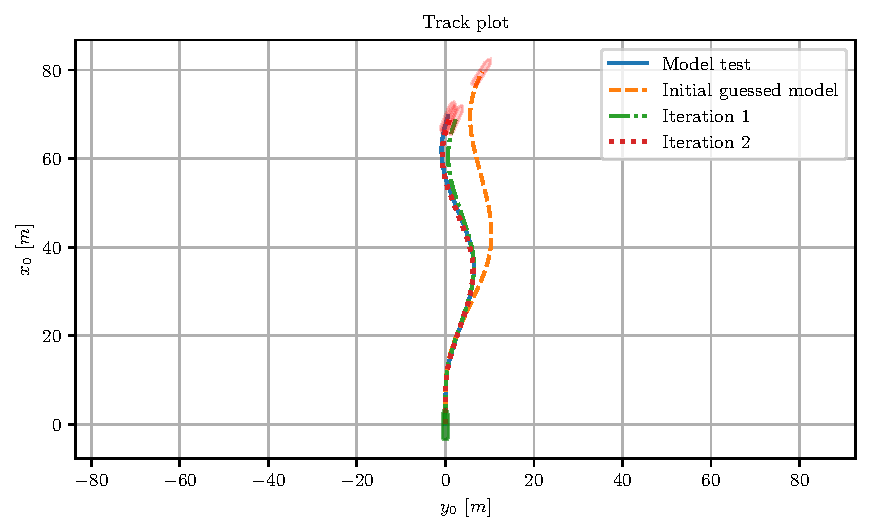
\includegraphics[width=\textwidth]{kappa/images/0.pdf}
    \caption{Simulation with: initial model, first and second iteration of the }
    \label{\detokenize{01.01_method:iterations}}
\end{figure}

\subsection{Inverse dynamics and regression}
\label{\detokenize{03.01_inverse_dynamics:inverse-dynamics-and-regression}}\label{\detokenize{03.01_inverse_dynamics::doc}}

Each manoeuvring model has some hydrodynamic functions \(X_D(u,v,r,\delta,thrust)\), \(Y_D(u,v,r,\delta,thrust)\), \(N_D(u,v,r,\delta,thrust)\) that are defined as polynomials. The hydrodynamic derivatives in these polynomials can be identified with force regression of measured forces and moments. The measured forces and moments are usually taken from Captive Model Tests (CMT), Planar Motion Mechanism (PMM) tests or Virtual Captive Tests (VCT). When the ship is free in all degrees of freedom, as in the present model tests, only
motions are recorded however. Hence, forces and moments causing ship motions need to be estimated by
solving the inverse dynamics problem.
The inverse dynamics is solved by restructuring the system equation (\autoref{equation:02.01_manoeuvring models:eqacc}) to get the hydrodynamics functions on the left-hand side. If the mass and inertia of the ship including added masses: \(X_{\dot{u}}\), \(Y_{\dot{v}}\), \(Y_{\dot{r}}\), \(N_{\dot{v}}\) and \(N_{\dot{r}}\), are known, the forces in Prime system can be calculated using \autoref{equation:03.01_inverse_dynamics:eqxd}, \autoref{equation:03.01_inverse_dynamics:eqyd} and \autoref{equation:03.01_inverse_dynamics:eqnd}.
These forces can be used to regress the hydrodynamic derivatives using the Ordinary Least Square (OLS) method. If the added masses are not known, they can be calculated with potential flow methods or semi-empirical methods (\autoref{app:initial_estimates}). 
\begin{equation}\label{equation:03.01_inverse_dynamics:eqxd}
\begin{split}\displaystyle \operatorname{X_{D}'}{\left(u',v',r',\delta,thrust' \right)} = - X_{\dot{u}}' \dot{u}' + \dot{u}' m' - m' r'^{2} x_{G}' - m' r' v'\end{split}
\end{equation}\begin{equation}\label{equation:03.01_inverse_dynamics:eqyd}
\begin{split}\displaystyle \operatorname{Y_{D}'}{\left(u',v',r',\delta,thrust' \right)} = - Y_{\dot{r}}' \dot{r}' - Y_{\dot{v}}' \dot{v}' + \dot{r}' m' x_{G}' + \dot{v}' m' + m' r' u'\end{split}
\end{equation}\begin{equation}\label{equation:03.01_inverse_dynamics:eqnd}
\begin{split}\displaystyle \operatorname{N_{D}'}{\left(u',v',r',\delta,thrust' \right)} = I_{z}' \dot{r}' - N_{\dot{r}}' \dot{r}' - N_{\dot{v}}' \dot{v}' + \dot{v}' m' x_{G}' + m' r' u' x_{G}'\end{split}
\end{equation}

\noindent An example of forces calculated with inverse dynamics from motions in a turning circle test can be seen in \hyperref[\detokenize{03.01_inverse_dynamics:fig-inverse}]{Fig.\@ \ref{\detokenize{03.01_inverse_dynamics:fig-inverse}}}. The forces have been converted to SI units.

\begin{figure}[H]
    \centering
    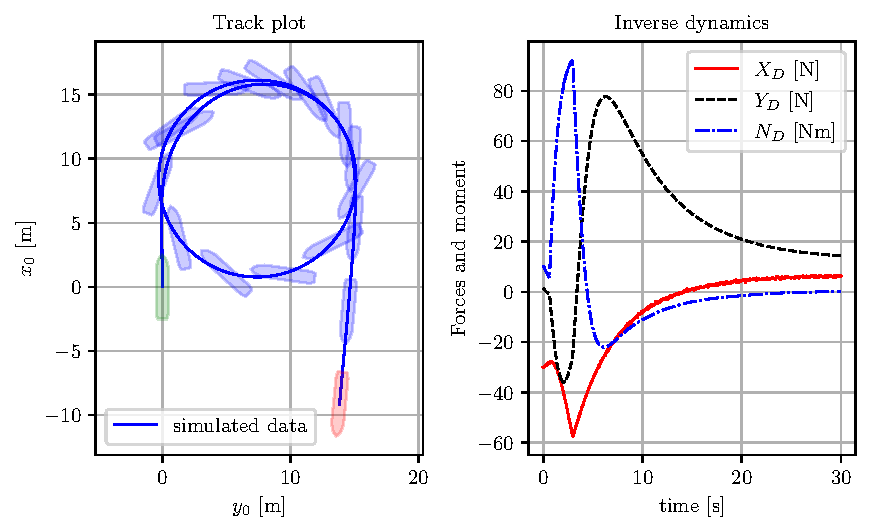
\includegraphics[width=\textwidth]{kappa/images/1.pdf}
    \caption{Example of forces and moments calculated with inverse dynamics on data from a turning circle test.}
    \label{\detokenize{03.01_inverse_dynamics:fig-inverse}}
\end{figure}

\subsection{Data cleaning}
\label{sec:datacleaning}
It is possible to do an exact parameter estimation on perfect (simulated) data with no noise (see Paper \ref{pap:daiyong} and \ref{pap:pit}). However, such data from physical experiments does not exist in reality. The measured data will always contain process noise and measurement noise. In order to mitigate this, the data is preprocessed using the Extended Kalman Filter (EKF) \cite{brown_introduction_1997} and Rauch Tung Striebel (RTS) smoother \cite{rauch_maximum_1965} which are both presented below.
EKF is an extension of the Kalman Filter (KF) to work on nonlinear systems such as the manoeuvring models. The basic idea is that noise can be disregarded if it does not make sense from a physical point of view. If noisy measurement data were perfectly correct, this would mean that the ship has many vibrations that must have originated from tremendous forces, considering the large mass of the ship. The prior understanding of the dynamics suggests that these forces are not present. Therefore, the noise should be considered as measurement noise and should be removed. Low-pass filtering is a common way to remove noise, where motions above some cut-off frequency are regarded as unphysical measurement noise. The problem with low-pass filter is that it is hard to know what cut-off frequency to choose, either too low: removing part of the signal, or too high: keeping some unfiltered measurement noise in the data. The Kalman filter has a system model, a manoeuvring model in this case, that continuously estimates the system’s state that runs in parallel with the measurement data. The filter estimates the current state as a combination of the measurement data and the system model estimate based on belief in the data and the model. If the data has low noise, the estimate turns toward that data. Conversely, if the model gives very good predictions, then that estimate turns towards the model.
The system’s inverse dynamics require the entire states, including positions, velocities, and accelerations, to be known. Only positions are known from the measurements, which means that velocities and accelerations are hidden states that the EKF can estimate.
The EKF is recursive and can be run online, continuously making new estimates as new measurements arrive. The EKF uses passed measurements to estimate states in the near future. This property is helpful for online applications such as  autopilots or autonomous ships. This restriction is  unnecessary for the estimation on already existing data where a whole time series of existing measurements is available. The fact that both past and future data are known can be used to improve the filter. An EKF filter can include future time steps by adding the RTS smoother after the filter. The RTS smoother is an algorithm that runs the EKF backward to also account for future time steps.

\subsection{Regression}
Finding the hydrodynamic derivatives can be defined as a linear regression problem:
\begin{equation}\label{equation:03.01_inverse_dynamics:eqregression}
\begin{split}y = X\gamma + \epsilon\end{split}
\end{equation}

\noindent A model for the hydrodynamic forces must first be assumed.
The label vector \(y\) and feature matrix \(X\) in the regression problem in \autoref{equation:03.01_inverse_dynamics:eqregression} can now be calculated, based on the assumed model. As an example: the label in the regression of the surge degree of freedom for the MAVMM can be calculated using the inverse dynamics force, expressed with primed units:
\begin{equation}\label{equation:03.01_inverse_dynamics:diff_eq_X_y}
\begin{split}\displaystyle y = - X_{\dot{u}} \dot{u}' + \dot{u}' m' - m' r'^{2} x_{G'} - m' r' v'\end{split}
\end{equation}

\noindent The feature matrix \(X\) is expressed as:
\begin{equation}\label{equation:03.01_inverse_dynamics:diff_eq_X_X}
\begin{split}\displaystyle X = \left[\begin{matrix}thrust' & u' & \delta^{2} & r'^{2} & u'^{2} & r' v'\end{matrix}\right]\end{split}
\end{equation}

\noindent The regressed hydrodynamic derivatives are stored in the \(\gamma\) vector:
\begin{equation}\label{equation:03.01_inverse_dynamics:diff_eq_X_beta}
\begin{split}\displaystyle \gamma = \left[\begin{matrix}X_{T}\\X_{u}\\X_{\delta\delta}\\X_{rr}\\X_{uu}\\X_{vr}\end{matrix}\right]\end{split}
\end{equation}

\noindent The hydrodynamic derivatives in the manoeuvring model are considered Gaussian random variables when conducting the Ordinary Least Squares (OLS) regression. The hydrodynamic derivatives in the manoeuvring model are usually taken as the mean value of each regressed random variable, being the most likely estimate. The regression result can be described with a Multivariate Gaussian Distribution, defined by the regression’s mean values and covariance matrix. Monte Carlo simulations can be conducted with this distribution to study alternative realizations of the regression.


Strong multicollinearity is a known problem for the manoeuvring models \cite{luo_parameter_2016}, \cite{wang_quantifying_2018}.
The thrust coefficient \(X_T\) in the hydrodynamic function \(X_D\) in \autoref{equation:02.01_manoeuvring models:eqxabkowitz} introduces multicollinearity to the regression. This coefficient can instead be calculated from the thrust deduction factor \(t_{df}\):
\begin{equation}\label{equation:03.01_inverse_dynamics:eqXthrust}
\begin{split}\displaystyle X_{T} = 1 - t_{df}\end{split}
\end{equation}

\noindent The \(X_T\) coefficient is excluded from the regression by moving it to the left-hand side of the regression equation \autoref{equation:03.01_inverse_dynamics:eqregression}:
\begin{equation}\label{equation:03.01_inverse_dynamics:eqexclude}
\begin{split}y-X_T \cdot thrust = X \gamma + \epsilon\end{split}
\end{equation}

\noindent Rudder coefficients (\(Y_R\)) from \(Y_D\) equation \autoref{equation:02.01_manoeuvring models:eqyabkowitz} such as \(Y_{\delta}\), \(Y_{\delta T}\) etc. have been excluded in the same way by assuming a connection with their \(N_D\) equation counterpart through the rudder lever arm \(x_r\):
\begin{equation}\label{equation:03.01_inverse_dynamics:eqyr}
\begin{split}\displaystyle Y_{R} = \frac{N_{R}}{x_{r'}}\end{split}
\end{equation}

\subsection{Model development process}
\label{sec:model_development_process}
The general aim of developing a manoeuvring model with parameter estimation is to develop a model that can generalize outside the known data. The method presented in this paper is evaluated with the holdout evaluation \cite{sammut_holdout_2017} where the data is divided into three sets: training set, validation set and test set as seen in \autoref{fig:model_development_process}.

\begin{figure}[H]
\centering
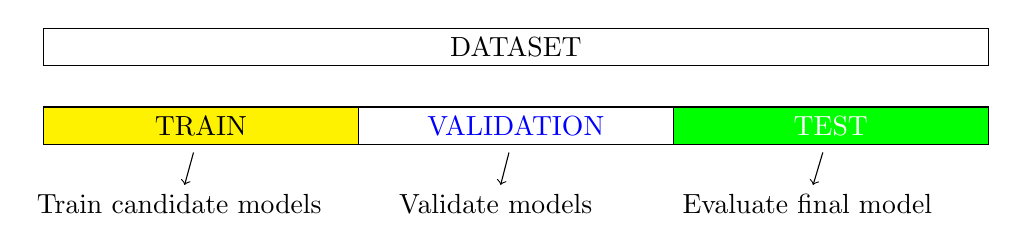
\begin{tikzpicture}

\node (dataset)[rectangle,
    anchor=west,
    draw,
    text = black,
    minimum width=12cm,
    fill = white] at (0, 0) {DATASET};

\node (train)[rectangle,
    draw,
    anchor=west,
    text = black,
    minimum width=4cm,
    fill = yellow] at (0, -1cm) {TRAIN};

\node (validation)[rectangle,
    draw,
    anchor=west,
    text = blue,
    minimum width=4cm,
    fill = white] at (4cm, -1cm) {VALIDATION};

\node (test)[rectangle,
    draw,
    anchor=west,
    text = white,
    minimum width=4cm,
    fill = green] at (8cm, -1cm){TEST};
    
\node (train_multiple)[rectangle,
    draw,
    anchor=west,
    text = black,
    draw = none,
    fill = none] at (-0.2cm, -2cm){Train candidate models};
    
\node (validate_models)[rectangle,
    draw,
    anchor=west,
    text = black,
    draw = none,
    fill = none] at (4.4cm, -2cm){Validate models};
    
\node (evaluate_models)[rectangle,
    draw,
    anchor=west,
    text = black,
    draw = none,
    fill = none] at (8.0cm, -2cm) {Evaluate final model};

\draw[shorten <=0.1cm,->] (train) -- (train_multiple);
\draw[shorten <=0.1cm,->] (validation) -- (validate_models);
\draw[shorten <=0.1cm,->] (test) -- (evaluate_models);
    
\end{tikzpicture}
\caption{Model development process with holdout evaluation}
\label{fig:model_development_process}
\end{figure}

\noindent The purpose with the training set is to train all the candidate models using the proposed parameter estimation method. The validation set is then used to select which one of the candidate models is the best. The training and validation sets are then joined to train the selected model as the final model, to be used in predicting the test set, which is used to evaluate the accuracy of the model. These three sets are not divided randomly, but rather to assess the model’s extrapolation ability. The data sets are therefore split to have the smallest: yaw rates, drift- and rudder-angles in the training set, the medium values in the validation set and the largest values in the test set which for instance can be seen in \autoref{fig:wpcc_datasets} in the next chapter.


